% This is a sample document using the University of Minnesota, Morris, Computer Science
% Senior Seminar modification of the ACM sig-alternate style. Much of this content is taken
% directly from the ACM sample document illustrating the use of the sig-alternate class. Certain
% parts that we never use have been removed to simplify the example, and a few additional
% components have been added.

% See https://github.com/UMM-CSci/Senior_seminar_templates for more info and to make
% suggestions and corrections.

\documentclass{sig-alternate}
\usepackage{color}
\usepackage[colorinlistoftodos]{todonotes}

%%%%% Uncomment the following line and comment out the previous one
%%%%% to remove all comments
%%%%% NOTE: comments still occupy a line even if invisible;
%%%%% Don't write them as a separate paragraph
%\newcommand{\mycomment}[1]{}

\begin{document}

% --- Author Metadata here ---
%%% REMEMBER TO CHANGE THE SEMESTER AND YEAR
\conferenceinfo{UMM CSci Senior Seminar Conference, December 2013}{Morris, MN}

\title{Usability of Error Messages for Introductory Students}

\numberofauthors{1}

\author{
% The command \alignauthor (no curly braces needed) should
% precede each author name, affiliation/snail-mail address and
% e-mail address. Additionally, tag each line of
% affiliation/address with \affaddr, and tag the
% e-mail address with \email.
\alignauthor
Paul A. Schliep\\
	\affaddr{Division of Science and Mathematics}\\
	\affaddr{University of Minnesota, Morris}\\
	\affaddr{Morris, Minnesota, USA 56267}\\
	\email{schli202@morris.umn.edu}
}

\maketitle
\begin{abstract}
Error messages are an important tool for programmers to help find and fix errors in their code. When an error message is unhelpful it can be difficult to understand how to find and fix the mistakes. Error messages are especially critical for introductory programmers in understanding problems with their code. Not all error messages are beneficial for helping novice programmers. This paper discusses how well error messages can help introductory students resolve mistakes in their programs and what aspects make an error message more user-friendly for introductory programmers. After that, we discuss the analyses of syntax, compiler, and exception errors and their results. We will also be discussing several methodologies and programs developed to help improve the experience a novice programmer has when attempting to understand causes for errors and their results.

% The current paper format *only* allows inline comments using the todo
% macro. That's kind of a bummer, and it would be neat if someone figured
% out how to change the acmconf style to allow this. I suspect it isn't *hard*
% but there are quite a few details that have to be sorted out in synchrony.
\todo[inline]{Will most likely be changing}
\end{abstract}

\keywords{Novice programmers, usability, error messages, usability studies, compiler errors, exception errors, syntax errors, functional-programming}


\section{Introduction}\label{intro}
One of the most important foundations of computer programming is the communication between the system and the user, specifically in the error messages produced by the system. These error messages are especially important for introductory-level computer science students to help them resolve issues in their program because the error messages are the primary source for understanding what's wrong and according to Marceau, "[they] lack the experience to decipher complicated or poorly-constructed feedback" ~\cite{Marceau:2011:MEE:1953163.1953308}. The first rule of good message design is to be sure that the error does not add confusion ~\cite{Isa:1983:MOE:800045.801583}. When a novice programmer receives an error message that they can not understand, it becomes difficult to fix their program. These difficulties often leads to frustration because the error message was either too complicated to understand or lead them down the wrong path~\cite{Marceau:2011:MYL:2048237.2048241}, which can sometimes introduce new errors ~\cite{Denny:2014:ESE:2591708.2591748}. 

Several studies have been conducted on modern programming languages' error messages to study the effectiveness in helping novice programmers debug their program and help learn the concepts and programming languages. The results have shown that students struggle with compiler and syntax error messages ~\cite{Denny:2014:ESE:2591708.2591748} ~\cite{Traver:2010} (which we will discuss in detail in Section 2) and the general vocabulary of the error messages along with IDE-specific features such as source highlighting can be bothersome for introductory computer science students ~\cite{Marceau:2011:MYL:2048237.2048241}. 

Several tools and heuristics are being developed to help address issues in error message usability and its development. The goals of these methodologies are to help introductory programmers learn the language and concepts easier. The goal of this paper is to discuss the analyses of error message design and its usability for introductory students in a classroom setting, and how these developed methodologies help improve the user experience with error messages. 

This paper is divided into five sections. In Section 2 we discuss usability studies, define compiler, syntax, and exception error messages, and discuss imperative and functional programming. In Section 3 we will focus on  analyses of the usability of exception messages and compiler messages for introductory students and how those analyses were performed. In Section 4 we discuss the results of those analyses. In Section 5 we discuss three methodologies developed to help improve the error message usability. The first we will discuss is Traver's heuristics for compiler message design ~\cite{Traver:2010}. Then, we will examine Marceau, Fisler, and Krishnamurthi's recommendations for error message design ~\cite{Marceau:2011:MYL:2048237.2048241}. Lastly, we will explore Denny, Luxton-Reilly, and Carpenter's syntax error enhancement tool ~\cite{Denny:2014:ESE:2591708.2591748}.

\todo[inline, color=orange]{Will most likely be changing}
\todo[inline, color=green]{Add image of error message example}


\section{Background}\label{background}
In order to discuss the analyses of error messages, we need to understand several concepts on error types and usability. These concepts include Compiler errors, Syntax errors, usability studies, and Human Computer Interaction (HCI). We will also be discussing the programming languages and tools whose error messages were analyzed. This includes Racket, C++, and Java programming languages and an overview of Integrated Development Environment (IDE) and DrRacket. 


\begin{itemize}
	\item Discuss Racket
	\item Discuss IDEs
	\item Discuss DrRacket
	\item Discuss C++
	\item Discuss Java
	\item Discuss Compiler errors
	\item Discuss Syntax errors
	\item Discuss parser
\end{itemize}

\subsection{Error Types}

\todo[inline, color=red]{TODO}

\subsection{Human-computer interaction and usability studies}

\todo[inline, color=red]{TODO}

\subsection{Overview of programming languages and tools analyzed}

\todo[inline, color=red]{TODO}


\section{Analyses}\label{analyses}
This section will discuss two different studies performed on the usability of error messages and what the results of those studies are. The first analysis will discuss how well the error messages in Racket and DrRacket help introductory students debug their programs. The second analysis will discuss the effectiveness of compiler error messages in the C++ programming language. 
\todo[inline, color=orange]{needs work}


\subsection{Analysis of error messages in Racket and DrRacket}
In the spring of 2010, Marceau, Fisler, and Krishnamurthi ran a usability study on error messages in DrRacket. The study involved configuring DrRacket to save a copy of each program a student tried to run as well as the error message through 6 50 minute lab sessions ~\cite{Marceau:2011:MEE:1953163.1953308}. The authors were interested in which error messages are effective and in what ways and how well DrRacket's text highlighting can help a student.  


In order to measure effectiveness, the authors developed a rubric which determined whether the student made a reasonable edit in response to the error message ~\cite{Marceau:2011:MEE:1953163.1953308}. The rubric was meant to distinguish how an error message would fail or succeed. They determined that an error message is effective if a student can read it, understand it, and use that information to figure out how to resolve the issue. 

Figure \ref{fig:racketerrormessage} shows an example of an error message in Racket that is not effective for a student. The message is contradicting itself as it does follow an open parenthesis, but the parser thinks the \texttt{and} is an independent part from the \texttt{cond}.

\begin{figure}[t!]
  \centering
  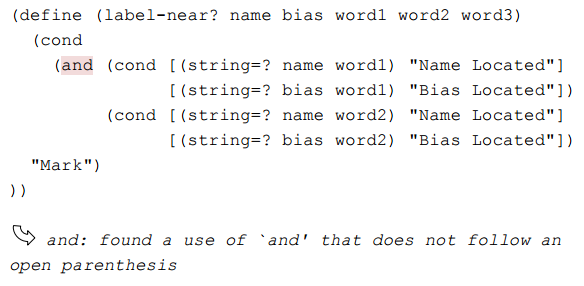
\includegraphics[keepaspectratio, width=0.55\textwidth]{MEE_example.png}
  \caption{Example of an ineffective error message in Racket}
  \label{fig:racketerrormessage}
\end{figure}

Marceau, Fisler, and Krishnamurthi grouped messages into nine most common error categories in their results from the study. Their rubric found the level of severity of the error messages. Through their data collection at the end of the study, they also found the level of occurrence of each error type from each lab and which error messages were poorly responded to, indicated as \textit{\%error} and \textit{\%bad}, respectively. \textit{\#bad} shows the level of likelihood of recurrence of the respective error message. The values of interest are the values enclosed in a box, which are the higher level \textit{\#bad} values, as seen in figure \ref{fig:drracketstudy}. 

The authors found from the data, that students have difficulties with certain errors at different points in the course. For example, in Lab 5 of the course, the authors found that the numerous argument count errors trace to mistakes in properly closing expressions. The error messages that the student saw from these mistakes did not match with the actual error the student encountered with their program. 


\begin{figure}[t!]
  \centering
  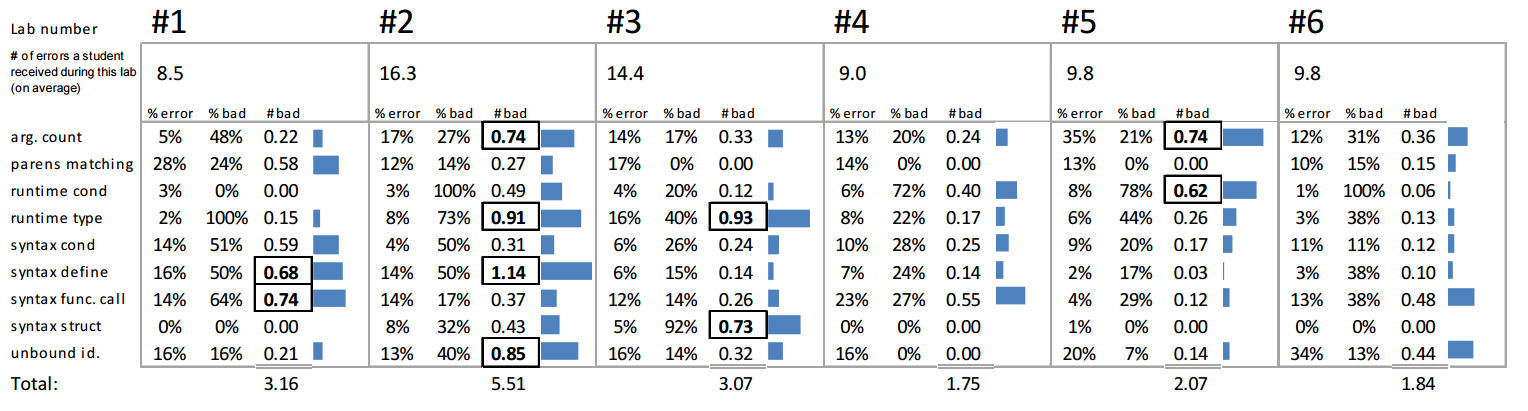
\includegraphics[keepaspectratio, width=0.55\textwidth]{MEE_Data.png}
  \caption{Results from DrRacket study}
  \label{fig:drracketstudy}
\end{figure}

\todo[inline, color=orange]{needs work}
\todo[inline, color=green]{add image of results from MEE, table 1, coding results}

\subsection{Analysis of compiler messages in C++}
Compiler error messages are often difficult to understand for many programmers, especially introductory programmers. 


\section{Methodologies}
In this section, we will be discussing three tools and methodologies meant to attempt to improve the usability of error messages or suggest improvements for error message design based on the results of the analyses discussed in section 3. The first methodology we will discuss is a set of recommendations for improving the usability of error messages. The second approach discusses improving compiler error messages through a set of principles meant to increase usability of the messages. For the third approach, we will discuss an attempt on enhancing syntax error messages in Java and the how well these syntax error messages improve over the original. 

\subsection{Recommendations for error messages}
This will use my source, Mind Your Language: On Novices' Interactions 
\todo[inline, color=red]{TODO}

\subsection{Principles of compiler error design}
This will use my source, On Compiler Error Messages: What They Say and What They Mean
\todo[inline, color=red]{TODO}

\subsection{Syntax error message enhancement and results}
This will use my source, Enhancing Syntax Error Messages Appears Ineffectual
\todo[inline, color=red]{TODO}


\section{Conclusion}
Discussion of the direction usability of error messages will be taken and how the methodologies will be applied for future work.

\todo[inline, color=red]{TODO}


\section{Acknowledgments}

\todo[inline, color=red]{TODO}


% The following two commands are all you need in the
% initial runs of your .tex file to
% produce the bibliography for the citations in your paper.
\bibliographystyle{acm}
% sample_paper.bib is the name of the BibTex file containing the
% bibliography entries. Note that you *don't* include the .bib ending here.
\bibliography{Usability_of_Error_Messages_for_Novice_Programmers}  

\todo[inline, color=blue]{Citing sources for references}
~\cite{Denny:2014:ESE:2591708.2591748}
~\cite{Hartmann:2010:OPS:1753326.1753478}
~\cite{Isa:1983:MOE:800045.801583}
~\cite{Marceau:2011:MEE:1953163.1953308}
~\cite{Marceau:2011:MYL:2048237.2048241}
~\cite{Murphy:2008:BTD:1352135.1352193}
~\cite{Traver:2010}
% You must have a proper ".bib" file
%  and remember to run:
% latex bibtex latex latex
% to resolve all references

\end{document}
